\documentclass{article}
\usepackage{listings}
\usepackage{color}
\usepackage{amsmath}
\usepackage{mathtools}
\usepackage{amsfonts}
\usepackage{amssymb}
\usepackage{caption}
\usepackage{tabularx}
\usepackage[export]{adjustbox}
\usepackage{polski}
\usepackage{indentfirst}
\usepackage{graphicx}
\usepackage{pdfpages}
\usepackage{float}
\usepackage{gauss}

\DeclareCaptionType{equ}[][List of equations]
\captionsetup[equ]{labelformat=empty}

%script adding bars in matrix
\usepackage{etoolbox}
\makeatletter
\patchcmd\g@matrix
 {\vbox\bgroup}
 {\vbox\bgroup\normalbaselines}% restore the standard baselineskip
 {}{}
\makeatother

\newcommand{\BAR}{%
  \hspace{-\arraycolsep}%
  \strut\vrule % the `\vrule` is as high and deep as a strut
  \hspace{-\arraycolsep}%
}
\definecolor{dkgreen}{rgb}{0,0.6,0}
\definecolor{gray}{rgb}{0.5,0.5,0.5}
\definecolor{mauve}{rgb}{0.58,0,0.82}

\lstset{frame=tb,
  language=Python,
  aboveskip=3mm,
  belowskip=3mm,
  showstringspaces=false,
  columns=flexible,
  basicstyle={\small\ttfamily},
  numbers=none,
  numberstyle=\tiny\color{gray},
  keywordstyle=\color{blue},
  commentstyle=\color{dkgreen},
  stringstyle=\color{mauve},
  breaklines=true,
  breakatwhitespace=true,
  tabsize=3,
  extendedchars=\true,
  inputencoding=utf8x
}

\lstset{literate={ą}{{\k{a}}}1 {ł}{{\l{}}}1 {ń}{{\'n}}1 {ę}{{\k{e}}}1 {ś}{{\'s}}1 {ż}{{\.z}}1 {ó}{{\'o}}1 {ź}{{\'z}}1 {Ą}{{\k{A}}}1 {Ł}{{\L{}}}1 {Ń}{{\'N}}1 {Ę}{{\k{E}}}1 {Ś}{{\'S}}1 {Ż}{{\.Z}}1 {Ó}{{\'O}}1 {Ź}{{\'Z}}1 }

\begin{document}
\title{Sprawozdanie - Metody numeryczne i optymailzacja}
\author{Jakub Andryszczak 259519,\\ Jakub Żak 244255,\\ Maciej Cierpisz 249163}
\date{}
\maketitle

\newpage
\tableofcontents
%Tutaj zaczyna się wstęp

\newpage
\section{Zadanie nr. 1}



\section{Zadanie nr. 2}

\section{Zadanie nr. 3}

Rozwiąż poniższy układ równań nieliniowych:\\
\begin{equation}
  \begin{cases}
    2x_1=x_2=exp(-x_1)\\
    -x_1+2x_2=exp(-x_2)
  \end{cases}
\end{equation}

dla punktu startowego $x_0=[-5 5]^t$.

Poniżej kod realizujący zadanie:

\begin{lstlisting}
  
  import numpy as np
  from scipy.optimize import fsolve
  
  # Define the system of nonlinear equations
  def equations(vars):
      x1, x2 = vars
      eq1 = 2 * x1 - x2 - np.exp(-x1)
      eq2 = -x1 + 2 * x2 - np.exp(-x2)
      return [eq1, eq2]
  
  # Initial guess
  x0 = [-5, -5]
  
  # Solve the system of equations
  solution = fsolve(equations, x0)
  
  # Print the solution
  print("Solution:")
  print(f"x1 = {solution[0]}")
  print(f"x2 = {solution[1]}")

\end{lstlisting}

Wyniki:

\begin{equation}
  \begin{cases}
    x_1=0.5671432904097838\\
    x_2=0.567143290409784
  \end{cases}
\end{equation}

\section{Zadanie nr. 4}
Znajdź rozwiązanie minimalizujące funkcję celu\\
$\sum_{k=1}^{10}(2+2k-exp(kx_1)-exp(kx_2))^2$\\
dla punktu początkowego $x_0=[0.3, 0.4]^T$.

Poniżej kod realizujący zadanie:

\begin{lstlisting}
  import numpy as np
from scipy.optimize import minimize

# Define the objective function
def objective(x):
    x1, x2 = x
    total = 0
    for k in range(1, 11):
        total += (2 + 2*k - np.exp(k*x1) - np.exp(k*x2))**2
    return total

# Initial guess
x0 = [0.3, 0.4]

# Minimize the objective function
result = minimize(objective, x0)

# Print the solution
print("Solution:")
print(f"x1 = {result.x[0]}")
print(f"x2 = {result.x[1]}")
\end{lstlisting}

Wyniki:

\begin{equation}
  \begin{cases}
    x_1=0.25782520984040996\\
    x_2=0.2578252098334402
  \end{cases}
\end{equation}

\section{Zadanie nr. 5}
Tłumienie fal elektromagnetycznych propagowanej w środowisku pozamiejskim w odległości \( d \) (w kilometrach) od stacji bazowej może być w przybliżeniu opisane modelem:
\[
L = 128.3 + 32.5 \log d + c, \quad [\text{dB}]
\]
gdzie \( c \sim \mathcal{N}(0, \sigma^2) \) odzwierciedla efekty tłumienia spowodowany przez zjawisko powolnego zanikania (slow fading). Niech \( c = 3 \) oraz \( d = [0.1, 0.2, \ldots, 10] \) [km]. Wykreśl tłumienie \( L \) w funkcji odległości \( d \) dla wybranych \( \sigma \). Następnie dopasuj modele:
\[
y = \alpha + \beta \log d, \quad \text{(logarytmiczny)}
\]
\[
y = \alpha + \beta d + \gamma d^2, \quad \text{(kwadratowy)}
\]
\[
y = \alpha + \beta d + \gamma d^2 + \delta d^3, \quad \text{(trzeciego stopnia)}
\]
do obserwowanych danych w sensie metryki najmniejszych kwadratów oraz wyznacz parametry \( \{ \alpha, \beta, \gamma, \delta \} \).
\newline

Do wykonania tego zadania posłużono się pythonem w celu wykreślenia wszystkich. 
\begin{lstlisting}
  import numpy as np
import matplotlib.pyplot as plt
from scipy.optimize import curve_fit

# Generowanie danych zgodnie z modelem
c = 3  # Stała wartość c zgodnie z zadaniem
d = np.arange(0.1, 10.1, 0.1)
L = 128.3 + 32.51 * np.log10(d) + c  # Dodajemy stałą wartość c

# Definicje modeli
def log_model(d, alpha, beta):
    return alpha + beta * np.log10(d)

def quadratic_model(d, alpha, beta, gamma):
    return alpha + beta * d + gamma * d**2

def cubic_model(d, alpha, beta, gamma, delta):
    return alpha + beta * d + gamma * d**2 + delta * d**3

# Dopasowanie modeli do danych
popt_log, _ = curve_fit(log_model, d, L)
popt_quad, _ = curve_fit(quadratic_model, d, L)
popt_cubic, _ = curve_fit(cubic_model, d, L)

# Predykcja przy użyciu dopasowanych modeli
L_log_fit = log_model(d, *popt_log)
L_quad_fit = quadratic_model(d, *popt_quad)
L_cubic_fit = cubic_model(d, *popt_cubic)

# Wykres danych i dopasowanych modeli
plt.figure(figsize=(10, 6))
plt.scatter(d, L, label='Dane', color='black')
plt.plot(d, L_log_fit, label='Model logarytmiczny', color='red')
plt.plot(d, L_quad_fit, label='Model kwadratowy', color='blue')
plt.plot(d, L_cubic_fit, label='Model trzeciego stopnia', color='green')
plt.xlabel('Odległość (d) [km]')
plt.ylabel('Tłumienie (L) [dB]')
plt.legend()
plt.title('Dopasowanie modeli tłumienia do danych')
plt.show()

# Wyświetlenie parametrów
print("Parametry modelu logarytmicznego: alpha = {:.4f}, beta = {:.4f}".format(*popt_log))
print("Parametry modelu kwadratowego: alpha = {:.4f}, beta = {:.4f}, gamma = {:.4f}".format(*popt_quad))
print("Parametry modelu trzeciego stopnia: alpha = {:.4f}, beta = {:.4f}, gamma = {:.4f}, delta = {:.4f}".format(*popt_cubic))
\end{lstlisting}
Wykonane wykresy oraz punkty powstały podstawiając do wzoru $L = 128.3 + 32.5logd+c$ za c = 3.
Powstałe wykresy prezentują się następująco:
\begin{figure}[h]
  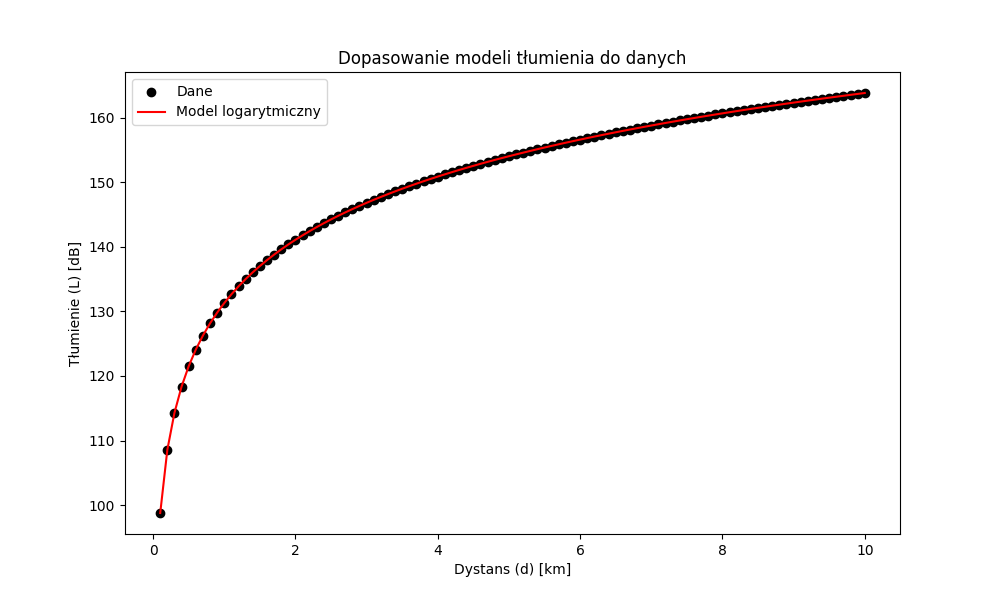
\includegraphics[scale=0.4]{logar3.png}
  \title{Rys 5.1 Wykres modelu logarytmicznego dopasowany do danych dla c stałego}
  \centering
\end{figure}
Parametry modelu logarytmicznego: $\alpha = 131.3000, \beta = 32.5100$\newpage
\begin{figure}[h]
  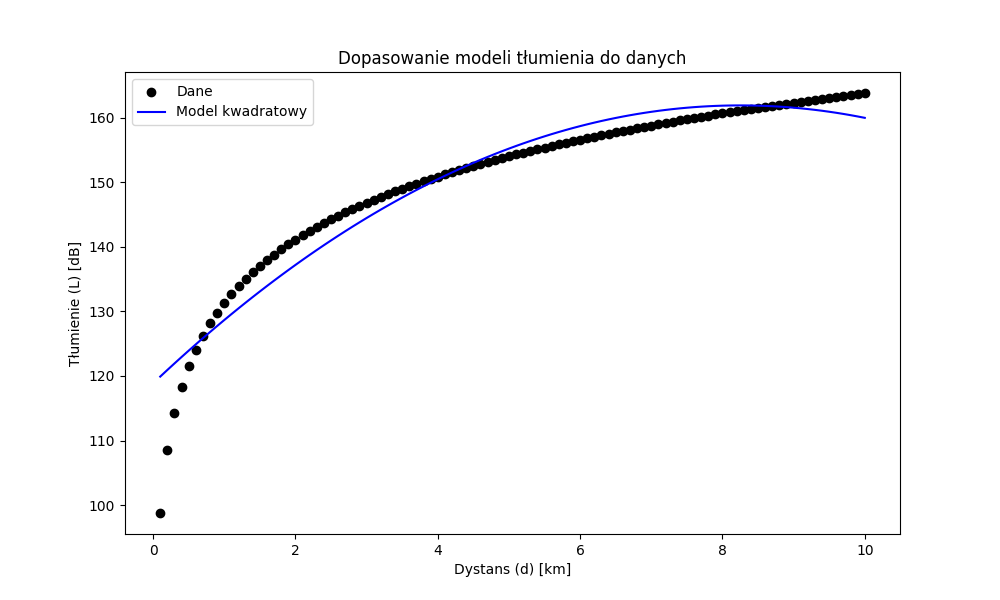
\includegraphics[scale=0.4]{kwadrat3.png}
  \title{Rys 5.2 Wykres modelu kwadratowego dopasowany do danych dla c stałego}
  \centering
\end{figure}
Parametry modelu kwadratowego: $\alpha = 118.8711, \beta = 10.4237, \gamma = -0.6314$\newpage
\begin{figure}[h]
  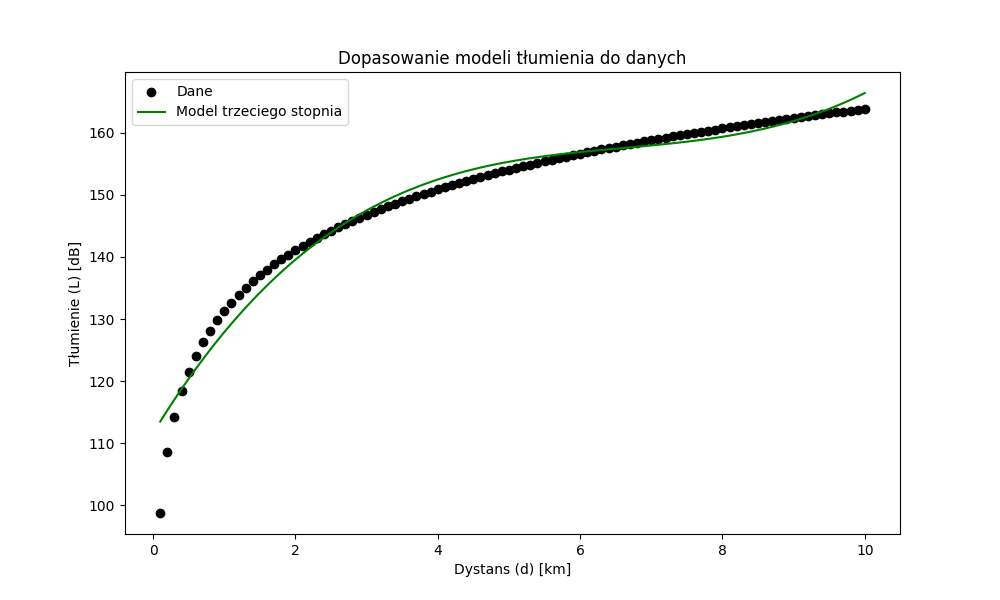
\includegraphics[scale=0.4]{trzy3.png}
  \title{Rys 5.3 Wykres modelu trzeciego stopnia dopasowany do danych dla c stałego}
  \centering
\end{figure}
Parametry modelu trzeciego stopnia: $\alpha = 111.6540, \beta = 18.7910, \gamma = -2.6923, \delta = 0.1360$ \newpage


W momencie gdy za c podstawimy $ \mathcal{N}(0, \sigma^2)$, a za $\sigma =1$ otrzymane wykresy i parametry modeli wyglądają następująco
\begin{figure}[h]
  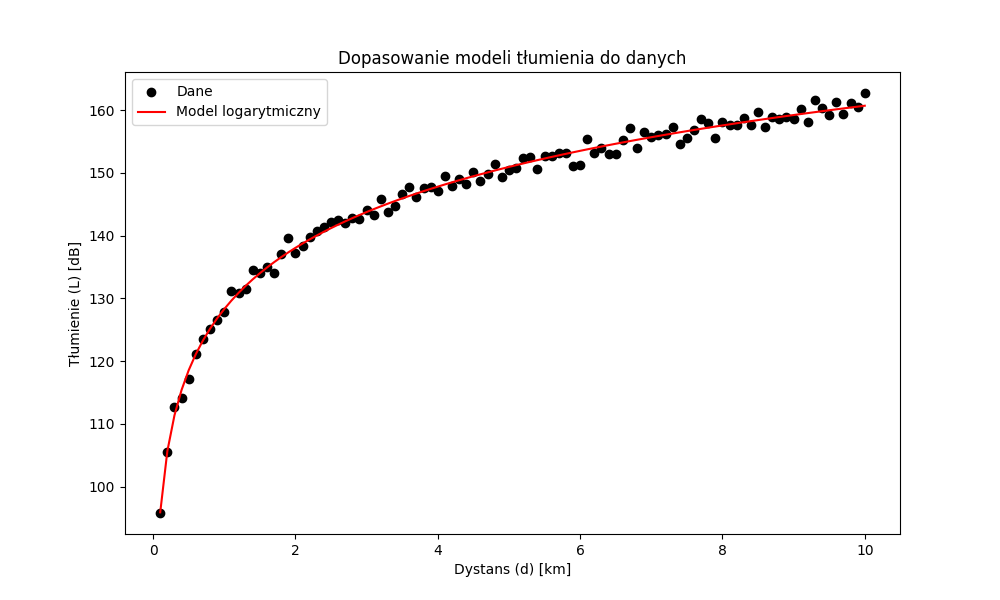
\includegraphics[scale=0.4]{logarN.png}
  \title{Rys 5.3 Wykres modelu logarytmicznego dopasowany do danych dla\( c \sim \mathcal{N}(0, \sigma^2) \)}
  \centering
\end{figure}
\newline
Parametry modelu logarytmicznego: $\alpha$ = 128.2009, $\beta$ = 32.6622 \newpage
\begin{figure}[h]
  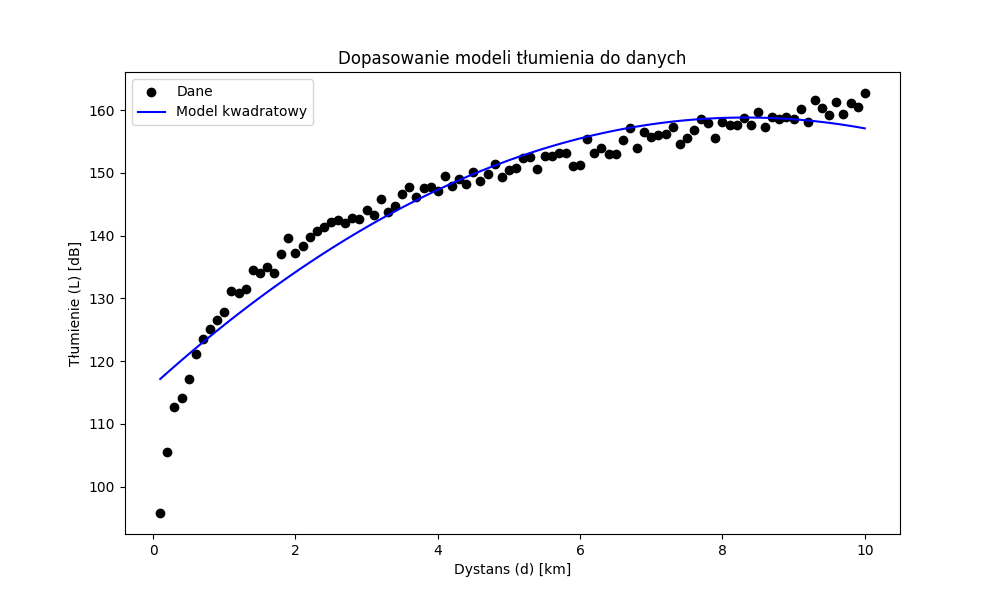
\includegraphics[scale=0.4]{kwadratN.png}
  \title{Rys 5.3 Wykres modelu kwadratowego dopasowany do danych dla \( c \sim \mathcal{N}(0, \sigma^2) \)}
  \centering
\end{figure}
Parametry modelu kwadratowego: alpha = 115.5702, beta = 10.5278, gamma = -0.6384 \newpage
\begin{figure}[h]
  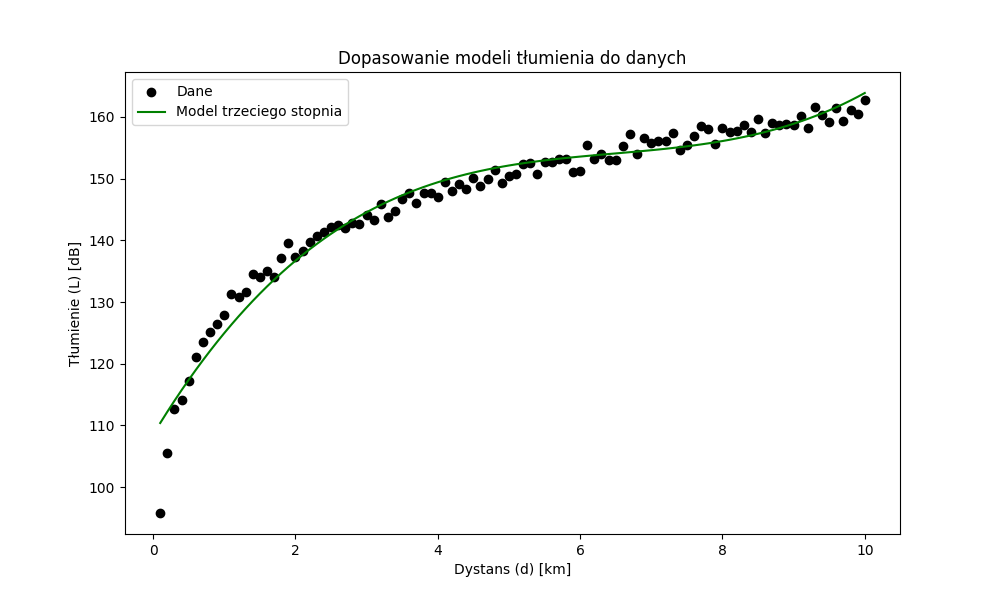
\includegraphics[scale=0.4]{trzyN.png}
  \title{Rys 5.3 Wykres modelu trzeciego stopnia dopasowany do danych dla \( c \sim \mathcal{N}(0, \sigma^2) \)}
  \centering
\end{figure}
 Parametry modelu trzeciego stopnia: alpha = 108.6487, beta = 18.5524, gamma = -2.6148, delta = 0.1305

 Dla wartości \( c \sim \mathcal{N}(0, \sigma^2) \) trudniej jest opisać, który z modeli jest dokładniejszy dla podanego zadania.
 Można jednak zauważyć, że w przypadku modelu logarytmicznego parametry pokrywają się z parametrami funkcji L.
 Jednak zakładając że c = 3, wartości stają się jeszcze bardziej dokładniejsze. Wychodzi wtedy, że model loarytmiczny idealnie sprawdza się w tym typie zadania, gdzie pozostałe lekko odbiegają od jego poprawności. 
 \end{document}